\documentclass[]{article}
\usepackage{lmodern}
\usepackage{amssymb,amsmath}
\usepackage{ifxetex,ifluatex}
\usepackage{fixltx2e} % provides \textsubscript
\ifnum 0\ifxetex 1\fi\ifluatex 1\fi=0 % if pdftex
  \usepackage[T1]{fontenc}
  \usepackage[utf8]{inputenc}
\else % if luatex or xelatex
  \ifxetex
    \usepackage{mathspec}
  \else
    \usepackage{fontspec}
  \fi
  \defaultfontfeatures{Ligatures=TeX,Scale=MatchLowercase}
\fi
% use upquote if available, for straight quotes in verbatim environments
\IfFileExists{upquote.sty}{\usepackage{upquote}}{}
% use microtype if available
\IfFileExists{microtype.sty}{%
\usepackage[]{microtype}
\UseMicrotypeSet[protrusion]{basicmath} % disable protrusion for tt fonts
}{}
\PassOptionsToPackage{hyphens}{url} % url is loaded by hyperref
\usepackage[unicode=true]{hyperref}
\hypersetup{
            pdfborder={0 0 0},
            breaklinks=true}
\urlstyle{same}  % don't use monospace font for urls
\usepackage{color}
\usepackage{fancyvrb}
\newcommand{\VerbBar}{|}
\newcommand{\VERB}{\Verb[commandchars=\\\{\}]}
\DefineVerbatimEnvironment{Highlighting}{Verbatim}{commandchars=\\\{\}}
% Add ',fontsize=\small' for more characters per line
\newenvironment{Shaded}{}{}
\newcommand{\KeywordTok}[1]{\textcolor[rgb]{0.00,0.44,0.13}{\textbf{#1}}}
\newcommand{\DataTypeTok}[1]{\textcolor[rgb]{0.56,0.13,0.00}{#1}}
\newcommand{\DecValTok}[1]{\textcolor[rgb]{0.25,0.63,0.44}{#1}}
\newcommand{\BaseNTok}[1]{\textcolor[rgb]{0.25,0.63,0.44}{#1}}
\newcommand{\FloatTok}[1]{\textcolor[rgb]{0.25,0.63,0.44}{#1}}
\newcommand{\ConstantTok}[1]{\textcolor[rgb]{0.53,0.00,0.00}{#1}}
\newcommand{\CharTok}[1]{\textcolor[rgb]{0.25,0.44,0.63}{#1}}
\newcommand{\SpecialCharTok}[1]{\textcolor[rgb]{0.25,0.44,0.63}{#1}}
\newcommand{\StringTok}[1]{\textcolor[rgb]{0.25,0.44,0.63}{#1}}
\newcommand{\VerbatimStringTok}[1]{\textcolor[rgb]{0.25,0.44,0.63}{#1}}
\newcommand{\SpecialStringTok}[1]{\textcolor[rgb]{0.73,0.40,0.53}{#1}}
\newcommand{\ImportTok}[1]{#1}
\newcommand{\CommentTok}[1]{\textcolor[rgb]{0.38,0.63,0.69}{\textit{#1}}}
\newcommand{\DocumentationTok}[1]{\textcolor[rgb]{0.73,0.13,0.13}{\textit{#1}}}
\newcommand{\AnnotationTok}[1]{\textcolor[rgb]{0.38,0.63,0.69}{\textbf{\textit{#1}}}}
\newcommand{\CommentVarTok}[1]{\textcolor[rgb]{0.38,0.63,0.69}{\textbf{\textit{#1}}}}
\newcommand{\OtherTok}[1]{\textcolor[rgb]{0.00,0.44,0.13}{#1}}
\newcommand{\FunctionTok}[1]{\textcolor[rgb]{0.02,0.16,0.49}{#1}}
\newcommand{\VariableTok}[1]{\textcolor[rgb]{0.10,0.09,0.49}{#1}}
\newcommand{\ControlFlowTok}[1]{\textcolor[rgb]{0.00,0.44,0.13}{\textbf{#1}}}
\newcommand{\OperatorTok}[1]{\textcolor[rgb]{0.40,0.40,0.40}{#1}}
\newcommand{\BuiltInTok}[1]{#1}
\newcommand{\ExtensionTok}[1]{#1}
\newcommand{\PreprocessorTok}[1]{\textcolor[rgb]{0.74,0.48,0.00}{#1}}
\newcommand{\AttributeTok}[1]{\textcolor[rgb]{0.49,0.56,0.16}{#1}}
\newcommand{\RegionMarkerTok}[1]{#1}
\newcommand{\InformationTok}[1]{\textcolor[rgb]{0.38,0.63,0.69}{\textbf{\textit{#1}}}}
\newcommand{\WarningTok}[1]{\textcolor[rgb]{0.38,0.63,0.69}{\textbf{\textit{#1}}}}
\newcommand{\AlertTok}[1]{\textcolor[rgb]{1.00,0.00,0.00}{\textbf{#1}}}
\newcommand{\ErrorTok}[1]{\textcolor[rgb]{1.00,0.00,0.00}{\textbf{#1}}}
\newcommand{\NormalTok}[1]{#1}
\usepackage{longtable,booktabs}
% Fix footnotes in tables (requires footnote package)
\IfFileExists{footnote.sty}{\usepackage{footnote}\makesavenoteenv{long table}}{}
\usepackage{graphicx,grffile}
\makeatletter
\def\maxwidth{\ifdim\Gin@nat@width>\linewidth\linewidth\else\Gin@nat@width\fi}
\def\maxheight{\ifdim\Gin@nat@height>\textheight\textheight\else\Gin@nat@height\fi}
\makeatother
% Scale images if necessary, so that they will not overflow the page
% margins by default, and it is still possible to overwrite the defaults
% using explicit options in \includegraphics[width, height, ...]{}
\setkeys{Gin}{width=\maxwidth,height=\maxheight,keepaspectratio}
\IfFileExists{parskip.sty}{%
\usepackage{parskip}
}{% else
\setlength{\parindent}{0pt}
\setlength{\parskip}{6pt plus 2pt minus 1pt}
}
\setlength{\emergencystretch}{3em}  % prevent overfull lines
\providecommand{\tightlist}{%
  \setlength{\itemsep}{0pt}\setlength{\parskip}{0pt}}
\setcounter{secnumdepth}{0}
% Redefines (sub)paragraphs to behave more like sections
\ifx\paragraph\undefined\else
\let\oldparagraph\paragraph
\renewcommand{\paragraph}[1]{\oldparagraph{#1}\mbox{}}
\fi
\ifx\subparagraph\undefined\else
\let\oldsubparagraph\subparagraph
\renewcommand{\subparagraph}[1]{\oldsubparagraph{#1}\mbox{}}
\fi

% set default figure placement to htbp
\makeatletter
\def\fps@figure{htbp}
\makeatother


\date{}

\begin{document}

\section{MIPS\_V2.0------多周期32位CPU}\label{header-n1821}

郑逸宁 15307130115

\tableofcontents

\subsubsection{一、项目概要}\label{header-n1826}

本次实验在上一次实验的基础,将CPU的单周期计算模式改进为多周期计算模式。多周期的原理非常简单,就是把每条指令拆分成若干个阶段,在每个时钟周期里执行一个阶段。因为不同指令的不同特性,有些指令可以通过较少的时钟周期来完成,这样当我们减少每个时钟周期的时间之后,整个CPU的执行效率就会加快。

整个多周期CPU的由一个状态机控制,每个状态表示了当前时钟周期在处理某种指令的某一阶段。每条指令的状态划分为IF,ID,EX,MEM和WB中的若干个,用``阶段\_指令类型''形式命名。由于我设计的多周期MIPS比基础要求多出了很多功能,所以在实验报告中只有文字描述的整体结构,不再使用结构图(因为真的太难画了)

\subsubsection{二、项目亮点}\label{header-n1831}

\begin{enumerate}
\def\labelenumi{\arabic{enumi}.}
\item
  使用了System Verilog这种较先进的硬件设计语言
\item
  多实现了beq,bne,lb,lbu,sb等指令,为设计64位指令积累经验(详见
  \textbf{\textless{}四、控制单元设计\textgreater{}})
\item
  所有组件使用参数化构建,便于下一步升级成64位CPU(详见
  \textbf{\textless{}五、数据通路设计\textgreater{}})
\item
  统一了数据存储器和指令存储器,实现了数据和指令的混合存储(详见
  \textbf{\textless{}六、存储器设计\textgreater{}})
\item
  使用\$display(),\$stop等命令,与波形图相结合进行仿真(详见
  \textbf{\textless{}七、测试\textgreater{}})
\item
  在Nexys4实验板上实现了:显示当前周期、显示当前阶段、查看任意内存、任意寄存器和随时暂停程序等全面的演示功能(详见
  \textbf{\textless{}八、演示设计\textgreater{}})
\end{enumerate}

\subsubsection{三、项目文件}\label{header-n1851}

根目录(/)

\begin{verbatim}
/bit/			存放各种版本的二进制文件(.bit)

/test/			存放各种版本的汇编文件(.s)、十六进制文件(.dat)

/images/		存放实验报告所需的图片(.png)

/source/		源代码(.sv)

.gitignore		git配置文件

memfile.dat		当前使用的十六进制文件

states.txt		Nexys4实验板演示说明

README.md		说明文档

Nexys4DDR_Master.xdc	Nexys4实验板引脚锁定文件

simulation_behav.wcfg	仿真波形图配置文件
\end{verbatim}

源代码(/source/)

\begin{verbatim}
alu.sv				ALU计算单元

aludec.sv 			ALU控制单元,用于输出alucontrol信号

clkdiv.sv 			时钟分频模块模块,用于演示

controller.sv 		mips的控制单元,包含maindec和aludec两部分

datapath.sv 		数据通路,mips的核心结构

flopenr.sv 			时钟控制的可复位触发寄存器

flopr.sv 			可复位触发寄存器

maindec.sv 			主控单元

mem.sv 				指令和数据的混合存储器

mips.sv				mips处理器的顶层模块

mux2.sv 			2:1复用器

mux3.sv 			3:1复用器

mux4.sv 			4:1复用器

mux5.sv 			5:1复用器

onboard.sv			在Nexys4实验板上测试的顶层模块

regfile.sv	 		寄存器文件

signext.sv 			符号拓展模块

simulation.sv 		仿真时使用的顶层模块

sl2.sv 				左移2位

top.sv 				包含mips和内存的顶层模块

zeroext.sv 			零拓展模块
\end{verbatim}

\subsubsection{四、状态机设计}\label{header-n1858}

多周期MIPS的核心是利用状态机表示当前CPU所处理的指令及这条指令正在处理的阶段,所以状态机的设计非常重要。根据所学的知识,我将每个指令拆分成IF、ID、EX、MEM和WB五个阶段中的若干阶段,并逐一设计出这些指令的不同阶段所要产生的控制信号。状态机如下表(其中EX\emph{LS
为Load和Store类指令共同的执行阶段,WB}L
为Load类指令共有的写回阶段,WB\_I为所有立即数计算指令共有的写回阶段):

\begin{longtable}[]{@{}llllll@{}}
\toprule
指令 & IF & ID & EX & MEM & WB\tabularnewline
\midrule
\endhead
RTYPE & IF & ID & EX\_RTYPE & & WB\_RTYPE\tabularnewline
LW & IF & ID & EX\_LS & MEM\_LW & WB\_L\tabularnewline
LBU & IF & ID & EX\_LS & MEM\_LBU & WB\_L\tabularnewline
LB & IF & ID & EX\_LS & MEM\_LB & WB\_L\tabularnewline
SW & IF & ID & EX\_LS & MEM\_SW &\tabularnewline
SB & IF & ID & EX\_LS & MEM\_SB &\tabularnewline
BEQ & IF & ID & EX\_BEQ & &\tabularnewline
BNE & IF & ID & EX\_BNE & &\tabularnewline
J & IF & ID & EX\_J & &\tabularnewline
ADDI & IF & ID & EX\_ADDI & & WB\_I\tabularnewline
ANDI & IF & ID & EX\_ANDI & & WB\_I\tabularnewline
ORI & IF & ID & EX\_ORI & & WB\_I\tabularnewline
SLTI & IF & ID & EX\_SLTI & & WB\_I\tabularnewline
\bottomrule
\end{longtable}

对于每个状态,我设计了21位的控制信号输出,他们分别是:

\begin{verbatim}
memwrite[1:0]	写存储器的类型,0表示不写,1表示写Word,2表示写Byte

pcwrite			用于计算pcen,pcen最后决定是否更新pc

irwrite			决定从存储器读出的数据是否当作指令进行译码

regwrite		是否写寄存器

alusrca			决定ALU的第一个运算数

branch			是否分支,用于计算pcen

iord			决定了从存储器读出的为指令还是数据

memtoreg		是否有从存储器到寄存器的数据存储

regdst			是否为R类指令

bne				是否为bne指令,用于计算pcen

alusrcb[2:0]	决定ALU的第二个运算数

pcsrc[1:0]		决定下一个pc的计算方式

aluop[2:0]		决定了alu计算的方式,传给aludec进行具体的控制

ltype[1:0]		读存储器的类型,0表示Word,1表示写Byte,2表示写UnsignedByte
\end{verbatim}

pcen的计算方式如下(其中zero表示ALU的计算结果是否为0):

\begin{Shaded}
\begin{Highlighting}[]
\CommentTok{/*controller.sv*/}
\KeywordTok{assign}\NormalTok{ pcen = pcwrite | (branch & zero) | (bne & ~zero);}
\end{Highlighting}
\end{Shaded}

对于不同状态的控制信号,在下面这段核心代码中给出:

\begin{Shaded}
\begin{Highlighting}[]
\CommentTok{/*maindec.sv*/}
\KeywordTok{assign}\NormalTok{ \{memwrite, pcwrite, irwrite, regwrite,}
\NormalTok{        alusrca, branch, iord, memtoreg, regdst,}
\NormalTok{        bne, alusrcb, pcsrc, aluop, ltype\} = controls; }
\NormalTok{always_comb	}
	\KeywordTok{case}\NormalTok{(state)}
            \DecValTok{IF:}\NormalTok{         controls <= }\BaseNTok{21'b00_110_00000_0_001_00_000_00}\NormalTok{;}
            \DecValTok{ID:}\NormalTok{         controls <= }\BaseNTok{21'b00_000_00000_0_011_00_000_00}\NormalTok{;}
            \DecValTok{EX_LS:}\NormalTok{      controls <= }\BaseNTok{21'b00_000_10000_0_010_00_000_00}\NormalTok{;}
            \DecValTok{MEM_LW:}\NormalTok{     controls <= }\BaseNTok{21'b00_000_00100_0_000_00_000_00}\NormalTok{;}
            \DecValTok{MEM_LB:}\NormalTok{     controls <= }\BaseNTok{21'b00_000_00100_0_000_00_000_10}\NormalTok{;}
            \DecValTok{MEM_LBU:}\NormalTok{    controls <= }\BaseNTok{21'b00_000_00100_0_000_00_000_01}\NormalTok{;}
            \DecValTok{WB_L:}\NormalTok{       controls <= }\BaseNTok{21'b00_001_00010_0_000_00_000_00}\NormalTok{;}
            \DecValTok{MEM_SW:}\NormalTok{     controls <= }\BaseNTok{21'b01_000_00100_0_000_00_000_00}\NormalTok{;}
            \DecValTok{MEM_SB:}\NormalTok{     controls <= }\BaseNTok{21'b10_000_00100_0_000_00_000_00}\NormalTok{;}
            \DecValTok{EX_RTYPE:}\NormalTok{   controls <= }\BaseNTok{21'b00_000_10000_0_000_00_010_00}\NormalTok{;}
            \DecValTok{WB_RTYPE:}\NormalTok{   controls <= }\BaseNTok{21'b00_001_00001_0_000_00_000_00}\NormalTok{;}
            \DecValTok{EX_BEQ:}\NormalTok{     controls <= }\BaseNTok{21'b00_000_11000_0_000_01_001_00}\NormalTok{;}
            \DecValTok{EX_BNE:}\NormalTok{     controls <= }\BaseNTok{21'b00_000_10000_1_000_01_001_00}\NormalTok{;}
            \DecValTok{EX_J:}\NormalTok{       controls <= }\BaseNTok{21'b00_100_00000_0_000_10_000_00}\NormalTok{;}
            \DecValTok{EX_ADDI:}\NormalTok{    controls <= }\BaseNTok{21'b00_000_10000_0_010_00_000_00}\NormalTok{;}
            \DecValTok{EX_ANDI:}\NormalTok{    controls <= }\BaseNTok{21'b00_000_10000_0_100_00_011_00}\NormalTok{; }
            \DecValTok{EX_ORI:}\NormalTok{     controls <= }\BaseNTok{21'b00_000_10000_0_100_00_100_00}\NormalTok{; }
            \DecValTok{EX_SLTI:}\NormalTok{    controls <= }\BaseNTok{21'b00_000_10000_0_010_00_101_00}\NormalTok{; }
            \DecValTok{WB_I:}\NormalTok{       controls <= }\BaseNTok{21'b00_001_00000_0_000_00_000_00}\NormalTok{;}
            \KeywordTok{default}\NormalTok{:    controls <= }\BaseNTok{21'b00_000_xxxxx_x_xxx_xx_xxx_xx}\NormalTok{;}
        \KeywordTok{endcase}
\end{Highlighting}
\end{Shaded}

ALU控制单元的设计和单周期MIPS一致,更多细节见如下三个源文件

\begin{verbatim}
controller.sv 
maindec.sv
aludec.sv
\end{verbatim}

\subsubsection{五、数据通路设计}\label{header-n1972}

\begin{figure}
\centering
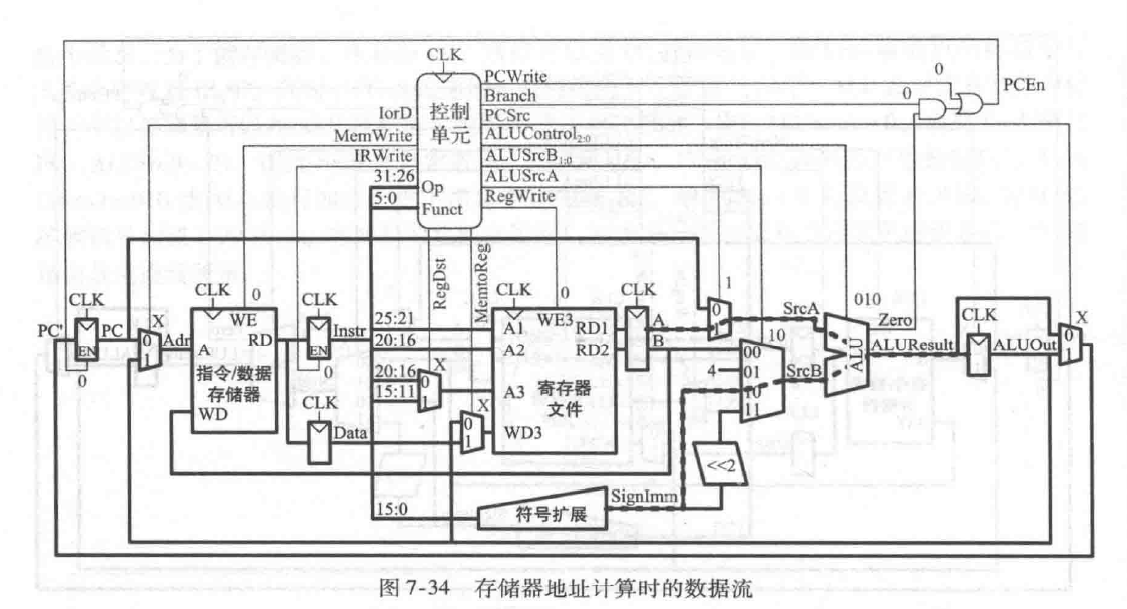
\includegraphics{C:/Users/will131/Documents/workspace/MIPS_V2.0/images/BaseOne.png}
\caption{}
\end{figure}

上面这张图是书上有一定功能的多周期MIPS的数据通路的示意图,支持\textbf{SW},\textbf{LW},\textbf{BEQ}和\textbf{R}类指令。通过选择合适的ALU运算数A和运算数B,可以用ALU来计算出下一条指令的可能的地址(分支后的地址、顺序下一条的地址),通过pcsrc选择其中之一,并用pcen来决定是否进行读取指令操作。然后通过iord来决定从存储器中读出的是指令还是数据,从而决定要读取寄存器的地址。其他流程与单周期MIPS类似,这里不再赘述。

\textbf{BEQ}指令和\textbf{BEQ}指令非常类似,我们只要增加一个控制信号bne来修改\textbf{BEQ}指令的数据流即可。

为了支持\textbf{J}指令,我们需要将pcsrc的值增加到3个选项,也就是将原来的2:1复用器变为3:1复用器,其中跳转后指令的地址由当前指令的低26位左移2位后拼接目前pc的高4位得到。具体的3:1复用器如下:

\begin{Shaded}
\begin{Highlighting}[]
\CommentTok{/*datapath.sv*/}
\NormalTok{mux3 #(N)       pcmux(aluresult, aluout, \{pc[}\DecValTok{31}\NormalTok{:}\DecValTok{28}\NormalTok{], instr[}\DecValTok{25}\NormalTok{:}\DecValTok{0}\NormalTok{], }\BaseNTok{2'b00}\NormalTok{\},pcsrc, pcnext);}
\end{Highlighting}
\end{Shaded}

上面的数据通路实际上也支持\textbf{ADDI}和\textbf{SLTI}两个指令,但我们为了增加对\textbf{ANDI}和\textbf{ORI}指令的支持,必须增加一个零扩展模块,作为ALU的运算数B的选择之一,所以我们需要把原来的4:1复用器,变为5:1复用器。具体的5:1复用器如下:

\begin{Shaded}
\begin{Highlighting}[]
\CommentTok{/*datapath.sv*/}
\NormalTok{mux5 #(N)       srcbmux(writedata, }\BaseNTok{32'b100}\NormalTok{, signimm, signimmsh, zeroimm, alusrcb, srcb);}
\end{Highlighting}
\end{Shaded}

最后,为了拓展\textbf{LB},\textbf{LBU}
这两个操作。我们对从存储区读出的数据进行选择,选择其中所需的Byte进行零拓展和符号拓展,再通过一个3:1复用器选择出,最后要使用的数据。这一块的实现如下:

\begin{Shaded}
\begin{Highlighting}[]
\CommentTok{/*datapath.sv*/}
\NormalTok{mux4 #(B)       lbmux(readdata[N-}\DecValTok{1}\NormalTok{:}\DecValTok{24}\NormalTok{], readdata[}\DecValTok{23}\NormalTok{:}\DecValTok{16}\NormalTok{], readdata[}\DecValTok{15}\NormalTok{:}\DecValTok{8}\NormalTok{],}
\NormalTok{                        readdata[}\DecValTok{7}\NormalTok{:}\DecValTok{0}\NormalTok{], aluout[}\DecValTok{1}\NormalTok{:}\DecValTok{0}\NormalTok{], mbyte);}
\NormalTok{zeroext #(B,N)  lbze(mbyte, mbytezext);}
\NormalTok{signext #(B,N)  lbse(mbyte, mbytesext);}
\NormalTok{mux3 #(N)       datamux(readdata, mbytezext, mbytesext, ltype, memdata);}
\end{Highlighting}
\end{Shaded}

数据通路的完整代码如下,其中使用了参数化设计,便于拓展位64位版本

\begin{Shaded}
\begin{Highlighting}[]
\CommentTok{/*datapath.sv*/}
\KeywordTok{module}\NormalTok{ datapath #(}\DataTypeTok{parameter}\NormalTok{ N = }\DecValTok{32}\NormalTok{, I = }\DecValTok{16}\NormalTok{ ,B = }\DecValTok{8}\NormalTok{)(}
    \DataTypeTok{input}\NormalTok{   logic       clk, reset,}
    \DataTypeTok{input}\NormalTok{   logic       pcen, irwrite,}
    \DataTypeTok{input}\NormalTok{   logic       regwrite,}
    \DataTypeTok{input}\NormalTok{   logic       iord, memtoreg, regdst, alusrca, }
    \DataTypeTok{input}\NormalTok{   logic [}\DecValTok{2}\NormalTok{:}\DecValTok{0}\NormalTok{] alusrcb,}
    \DataTypeTok{input}\NormalTok{   logic [}\DecValTok{1}\NormalTok{:}\DecValTok{0}\NormalTok{] pcsrc,}
    \DataTypeTok{input}\NormalTok{   logic [}\DecValTok{2}\NormalTok{:}\DecValTok{0}\NormalTok{] alucontrol,}
    \DataTypeTok{input}\NormalTok{   logic [}\DecValTok{1}\NormalTok{:}\DecValTok{0}\NormalTok{] ltype,}
    \DataTypeTok{output}\NormalTok{  logic [}\DecValTok{5}\NormalTok{:}\DecValTok{0}\NormalTok{] op, funct,}
    \DataTypeTok{output}\NormalTok{  logic       zero,}
    \DataTypeTok{output}\NormalTok{  logic [N-}\DecValTok{1}\NormalTok{:}\DecValTok{0}\NormalTok{]dataadr, writedata,}
    \DataTypeTok{input}\NormalTok{   logic [N-}\DecValTok{1}\NormalTok{:}\DecValTok{0}\NormalTok{]readdata,}
    \DataTypeTok{output}\NormalTok{  logic [}\DecValTok{7}\NormalTok{:}\DecValTok{0}\NormalTok{]  pclow,}
    \DataTypeTok{input}\NormalTok{   logic [}\DecValTok{4}\NormalTok{:}\DecValTok{0}\NormalTok{]  checka,}
    \DataTypeTok{output}\NormalTok{  logic [N-}\DecValTok{1}\NormalTok{:}\DecValTok{0}\NormalTok{]check}
\NormalTok{);}
\NormalTok{    logic [}\DecValTok{4}\NormalTok{:}\DecValTok{0}\NormalTok{]     writereg;}
\NormalTok{    logic [N-}\DecValTok{1}\NormalTok{:}\DecValTok{0}\NormalTok{]   pcnext, pc;}
\NormalTok{    logic [N-}\DecValTok{1}\NormalTok{:}\DecValTok{0}\NormalTok{]   instr, data, srca, srcb;}
\NormalTok{    logic [N-}\DecValTok{1}\NormalTok{:}\DecValTok{0}\NormalTok{]   rda;}
\NormalTok{    logic [N-}\DecValTok{1}\NormalTok{:}\DecValTok{0}\NormalTok{]   aluresult, aluout;}
\NormalTok{    logic [N-}\DecValTok{1}\NormalTok{:}\DecValTok{0}\NormalTok{]   signimm; }
\NormalTok{    logic [N-}\DecValTok{1}\NormalTok{:}\DecValTok{0}\NormalTok{]   zeroimm; }
\NormalTok{    logic [N-}\DecValTok{1}\NormalTok{:}\DecValTok{0}\NormalTok{]   signimmsh; }
\NormalTok{    logic [N-}\DecValTok{1}\NormalTok{:}\DecValTok{0}\NormalTok{]   wd3, rd1, rd2;}
\NormalTok{    logic [N-}\DecValTok{1}\NormalTok{:}\DecValTok{0}\NormalTok{]   memdata, mbytezext, mbytesext; }
\NormalTok{    logic [B-}\DecValTok{1}\NormalTok{:}\DecValTok{0}\NormalTok{]   mbyte;}
    \KeywordTok{assign}\NormalTok{ op = instr[N-}\DecValTok{1}\NormalTok{:}\DecValTok{26}\NormalTok{];}
    \KeywordTok{assign}\NormalTok{ funct = instr[}\DecValTok{5}\NormalTok{:}\DecValTok{0}\NormalTok{];}
    \KeywordTok{assign}\NormalTok{ pclow = pc[}\DecValTok{9}\NormalTok{:}\DecValTok{2}\NormalTok{];}
\NormalTok{    flopenr #(N)    pcreg(clk, reset, pcen, pcnext, pc);}
\NormalTok{    mux2 #(N)       adrmux(pc, aluout, iord, dataadr);}
\NormalTok{    flopenr #(N)    instrreg(clk, reset, irwrite, readdata, instr);}
\NormalTok{    mux4 #(B)       lbmux(readdata[N-}\DecValTok{1}\NormalTok{:}\DecValTok{24}\NormalTok{], readdata[}\DecValTok{23}\NormalTok{:}\DecValTok{16}\NormalTok{], readdata[}\DecValTok{15}\NormalTok{:}\DecValTok{8}\NormalTok{],}
\NormalTok{                        readdata[}\DecValTok{7}\NormalTok{:}\DecValTok{0}\NormalTok{], aluout[}\DecValTok{1}\NormalTok{:}\DecValTok{0}\NormalTok{], mbyte);}
\NormalTok{    zeroext #(B,N)  lbze(mbyte, mbytezext);}
\NormalTok{    signext #(B,N)  lbse(mbyte, mbytesext);}
\NormalTok{    mux3 #(N)       datamux(readdata, mbytezext, mbytesext, ltype, memdata);}
\NormalTok{    flopr #(N)      datareg(clk, reset, memdata, data);}
\NormalTok{    mux2 #(}\DecValTok{5}\NormalTok{)       regdstmux(instr[}\DecValTok{20}\NormalTok{:}\DecValTok{16}\NormalTok{],instr[}\DecValTok{15}\NormalTok{:}\DecValTok{11}\NormalTok{], regdst, writereg);}
\NormalTok{    mux2 #(N)       wdmux(aluout, data, memtoreg, wd3);}
\NormalTok{    regfile#(N,}\DecValTok{32}\NormalTok{)  regfile(clk, regwrite, instr[}\DecValTok{25}\NormalTok{:}\DecValTok{21}\NormalTok{], instr[}\DecValTok{20}\NormalTok{:}\DecValTok{16}\NormalTok{],}
\NormalTok{                        writereg, wd3, rd1, rd2, checka, check);}
\NormalTok{    flopr #(N)      rdareg(clk, reset, rd1, rda);}
\NormalTok{    flopr #(N)      wdreg(clk, reset, rd2, writedata);}
\NormalTok{    signext#(I,N)   signext(instr[}\DecValTok{15}\NormalTok{:}\DecValTok{0}\NormalTok{], signimm);}
\NormalTok{    zeroext#(I,N)   zeroext(instr[}\DecValTok{15}\NormalTok{:}\DecValTok{0}\NormalTok{], zeroimm);}
\NormalTok{    sl2             immsh(signimm, signimmsh);}
\NormalTok{    mux2 #(N)       srcamux(pc, rda, alusrca, srca);}
\NormalTok{    mux5 #(N)       srcbmux(writedata, }\BaseNTok{32'b100}\NormalTok{, signimm, signimmsh, zeroimm, alusrcb, srcb);}
\NormalTok{    alu             alu(srca, srcb, alucontrol, aluresult, zero);}
\NormalTok{    flopr #(N)      alureg(clk, reset, aluresult, aluout);}
\NormalTok{    mux3 #(N)       pcmux(aluresult, aluout, \{pc[}\DecValTok{31}\NormalTok{:}\DecValTok{28}\NormalTok{], instr[}\DecValTok{25}\NormalTok{:}\DecValTok{0}\NormalTok{], }\BaseNTok{2'b00}\NormalTok{\},pcsrc, pcnext);}
\KeywordTok{endmodule}
\end{Highlighting}
\end{Shaded}

\subsubsection{六、存储器设计}\label{header-n1991}

我在对存储器的设计上选择了参数化实现,设定了单元的大小N和单元数L。目前N=32,L=256,即以字为基本单元。后续改进中会设定N=64,即以双字为基本单元。我实现了在存储器上写字(SW)、写半字(SH)和写位(SB)的操作,类似的操作可以应用到N=64的情况,可以说是为下一步的改进打下了基础。存储器的完整代码如下:

\begin{Shaded}
\begin{Highlighting}[]
\CommentTok{/*mem.sv*/}
\KeywordTok{module}\NormalTok{ mem#(}\DataTypeTok{parameter}\NormalTok{ N = }\DecValTok{32}\NormalTok{, L = }\DecValTok{256}\NormalTok{)(}
    \DataTypeTok{input}\NormalTok{   logic           clk, }
    \DataTypeTok{input}\NormalTok{   logic [}\DecValTok{1}\NormalTok{:}\DecValTok{0}\NormalTok{]     memwrite,}
    \DataTypeTok{input}\NormalTok{   logic [N-}\DecValTok{1}\NormalTok{:}\DecValTok{0}\NormalTok{]   dataadr, writedata,}
    \DataTypeTok{output}\NormalTok{  logic [N-}\DecValTok{1}\NormalTok{:}\DecValTok{0}\NormalTok{]   readdata,}
    \DataTypeTok{input}\NormalTok{   logic [}\DecValTok{7}\NormalTok{:}\DecValTok{0}\NormalTok{]     checka,}
    \DataTypeTok{output}\NormalTok{  logic [N-}\DecValTok{1}\NormalTok{:}\DecValTok{0}\NormalTok{]   check}
\NormalTok{);}
\NormalTok{    logic [N-}\DecValTok{1}\NormalTok{:}\DecValTok{0}\NormalTok{] RAM [L-}\DecValTok{1}\NormalTok{:}\DecValTok{0}\NormalTok{];}
    \KeywordTok{initial}
        \DataTypeTok{$readmemh}\NormalTok{(}\StringTok{"C:/Users/will131/Documents/workspace/MIPS_V2.0/memfile.dat"}\NormalTok{,RAM);}
    \KeywordTok{assign}\NormalTok{ readdata = RAM[dataadr[N-}\DecValTok{1}\NormalTok{:}\DecValTok{2}\NormalTok{]];}
    \KeywordTok{assign}\NormalTok{ check = RAM[checka];}
    \KeywordTok{always}\NormalTok{ @(}\KeywordTok{posedge}\NormalTok{ clk)}
        \KeywordTok{begin}
        \KeywordTok{if}\NormalTok{ (memwrite===}\DecValTok{1}\NormalTok{)}
\NormalTok{            RAM[dataadr[N-}\DecValTok{1}\NormalTok{:}\DecValTok{2}\NormalTok{]] <= writedata;}
        \KeywordTok{else} \KeywordTok{if}\NormalTok{ (memwrite===}\DecValTok{2}\NormalTok{) }\CommentTok{//B}
                \KeywordTok{case}\NormalTok{ (dataadr[}\DecValTok{1}\NormalTok{:}\DecValTok{0}\NormalTok{])}
                    \BaseNTok{2'b11}\NormalTok{:  RAM[dataadr[N-}\DecValTok{1}\NormalTok{:}\DecValTok{2}\NormalTok{]][}\DecValTok{7}\NormalTok{:}\DecValTok{0}\NormalTok{]  <= writedata[}\DecValTok{7}\NormalTok{:}\DecValTok{0}\NormalTok{];}
                    \BaseNTok{2'b10}\NormalTok{:  RAM[dataadr[N-}\DecValTok{1}\NormalTok{:}\DecValTok{2}\NormalTok{]][}\DecValTok{15}\NormalTok{:}\DecValTok{8}\NormalTok{] <= writedata[}\DecValTok{7}\NormalTok{:}\DecValTok{0}\NormalTok{];}
                    \BaseNTok{2'b01}\NormalTok{:  RAM[dataadr[N-}\DecValTok{1}\NormalTok{:}\DecValTok{2}\NormalTok{]][}\DecValTok{23}\NormalTok{:}\DecValTok{16}\NormalTok{]<= writedata[}\DecValTok{7}\NormalTok{:}\DecValTok{0}\NormalTok{];}
                    \BaseNTok{2'b00}\NormalTok{:  RAM[dataadr[N-}\DecValTok{1}\NormalTok{:}\DecValTok{2}\NormalTok{]][}\DecValTok{31}\NormalTok{:}\DecValTok{24}\NormalTok{]<= writedata[}\DecValTok{7}\NormalTok{:}\DecValTok{0}\NormalTok{];}
                \KeywordTok{endcase}
        \KeywordTok{else} \KeywordTok{if}\NormalTok{ (memwrite===}\DecValTok{3}\NormalTok{) }\CommentTok{//H}
            \KeywordTok{case}\NormalTok{ (dataadr[}\DecValTok{1}\NormalTok{])}
                    \DecValTok{1}\NormalTok{:  RAM[dataadr[N-}\DecValTok{1}\NormalTok{:}\DecValTok{2}\NormalTok{]][}\DecValTok{15}\NormalTok{:}\DecValTok{0}\NormalTok{]  <= writedata[}\DecValTok{15}\NormalTok{:}\DecValTok{0}\NormalTok{];}
                    \DecValTok{0}\NormalTok{:  RAM[dataadr[N-}\DecValTok{1}\NormalTok{:}\DecValTok{2}\NormalTok{]][}\DecValTok{31}\NormalTok{:}\DecValTok{16}\NormalTok{] <= writedata[}\DecValTok{15}\NormalTok{:}\DecValTok{0}\NormalTok{];}
                \KeywordTok{endcase}
        \KeywordTok{end} 
\KeywordTok{endmodule}
\end{Highlighting}
\end{Shaded}

\subsubsection{七、测试}\label{header-n1995}

我设计了三个程序,结合书上的程序进行测试,他们的大致内容如下,具体代码见test文件夹:

\begin{verbatim}
standard		书上的测试程序
standard2		测试除LB,LBU,SB外的15条指令的正确性
power2			生成2的次幂,并存在存储器中,主要用于演示
testls			测试LB,LBU,SB,测试数据和指令混合
\end{verbatim}

standard2的部分波形图如下,可以查看存储器的变化、状态机中状态的变化和ALU的计算结果等。

\begin{figure}
\centering
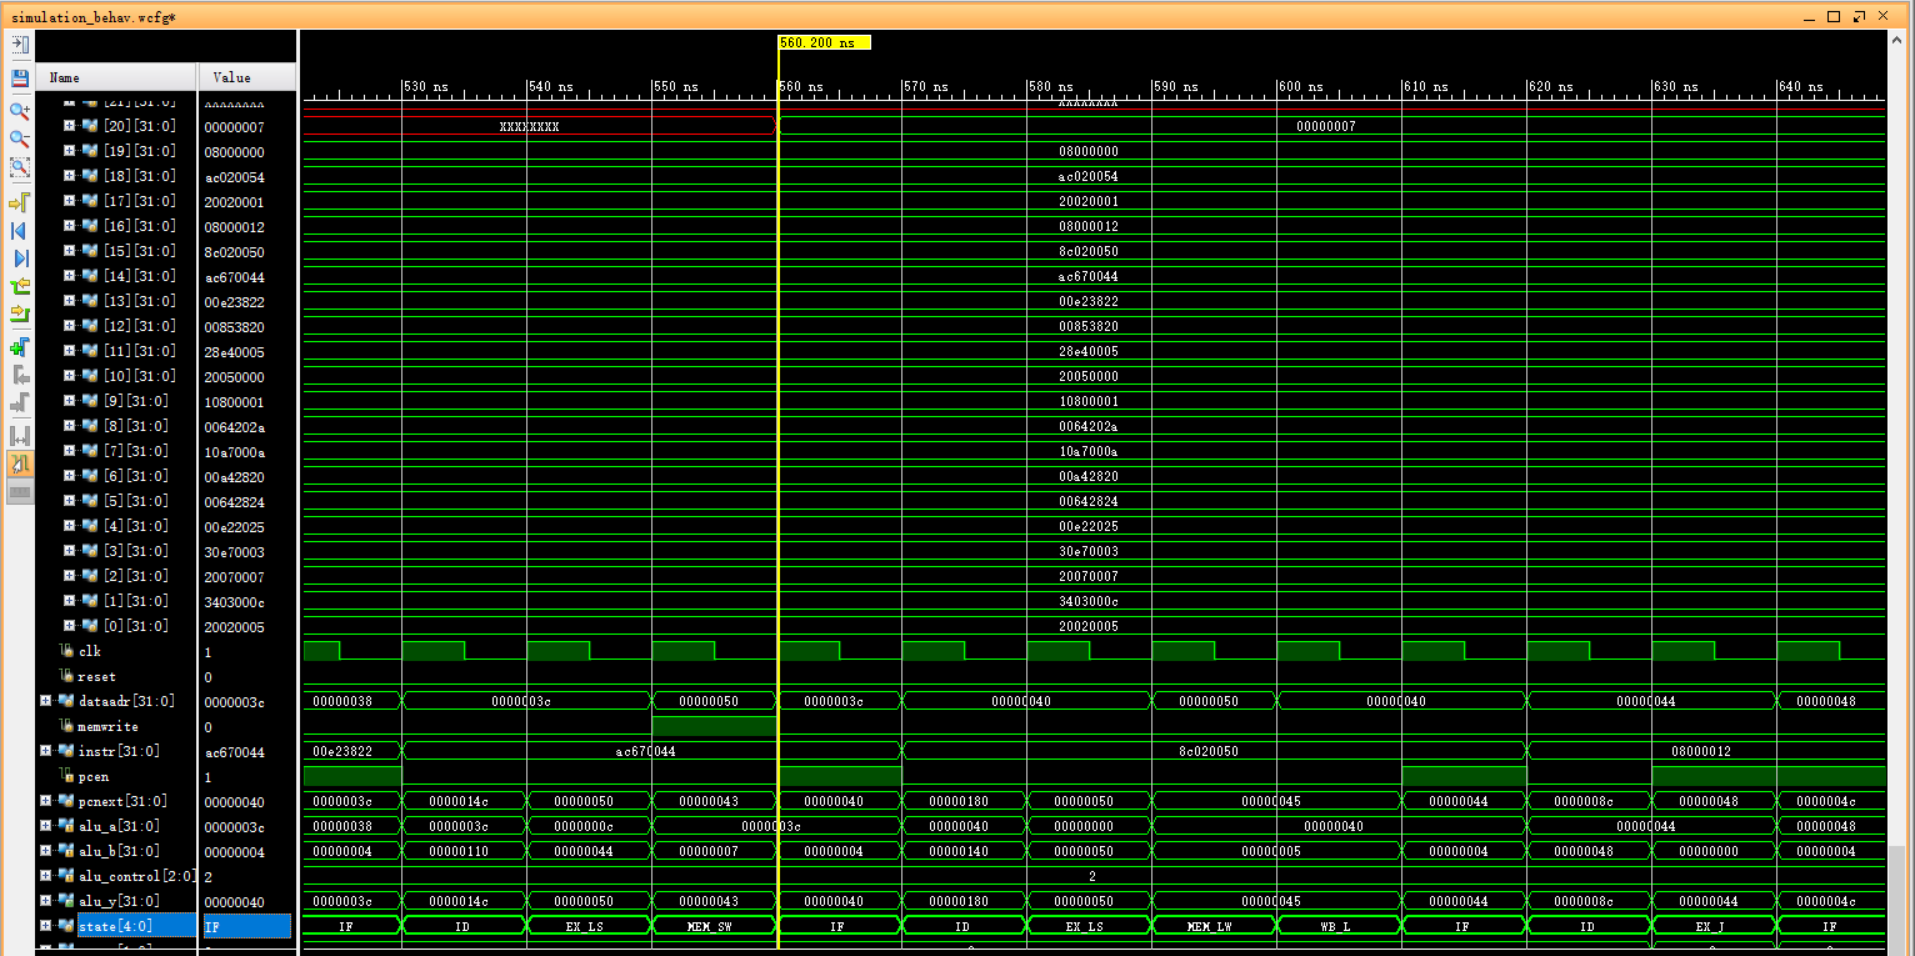
\includegraphics{C:/Users/will131/Documents/workspace/MIPS_V2.0/images/Simulation.png}
\caption{}
\end{figure}

我同时通过\$display()输出每个寄存器的变化来验证我程序的正确性。程序正确结束时会停在我们预设的\$stop的位置。实现这些测试的核心代码在如下两处:

\begin{Shaded}
\begin{Highlighting}[]
\CommentTok{/*regfile.sv*/}
\NormalTok{always_ff @(}\KeywordTok{posedge}\NormalTok{ clk)}
    \KeywordTok{if}\NormalTok{ (we3) }\KeywordTok{begin}
        \DataTypeTok{$display}\NormalTok{(}\StringTok{"REG%d=%d"}\NormalTok{,wa3,wd3);}
\NormalTok{        rf[wa3] <= wd3;}
    \KeywordTok{end}

\CommentTok{/*simulation.sv*/}
\KeywordTok{always}\NormalTok{ @(}\KeywordTok{negedge}\NormalTok{ clk) }\KeywordTok{begin}
    \KeywordTok{if}\NormalTok{ (memwrite) }\KeywordTok{begin}
        \KeywordTok{if}\NormalTok{ (dataadr === }\DecValTok{84}\NormalTok{ & writedata === }\DecValTok{7}\NormalTok{)}\KeywordTok{begin}
            \DataTypeTok{$display}\NormalTok{(}\StringTok{"LOG:Simulation succeeded"}\NormalTok{);}
            \DataTypeTok{$stop}\NormalTok{;}
        \KeywordTok{end}
    \KeywordTok{end}
\NormalTok{    cnt = cnt + }\DecValTok{1}\NormalTok{;}
    \KeywordTok{if}\NormalTok{(cnt === }\DecValTok{128}\NormalTok{)}
        \DataTypeTok{$stop}\NormalTok{;}
\KeywordTok{end}
\end{Highlighting}
\end{Shaded}

testls.s的部分波形图如下,可以看到程序读出了存储器中下标为5的字的前两位,相加后存放在了第四位。

\begin{figure}
\centering
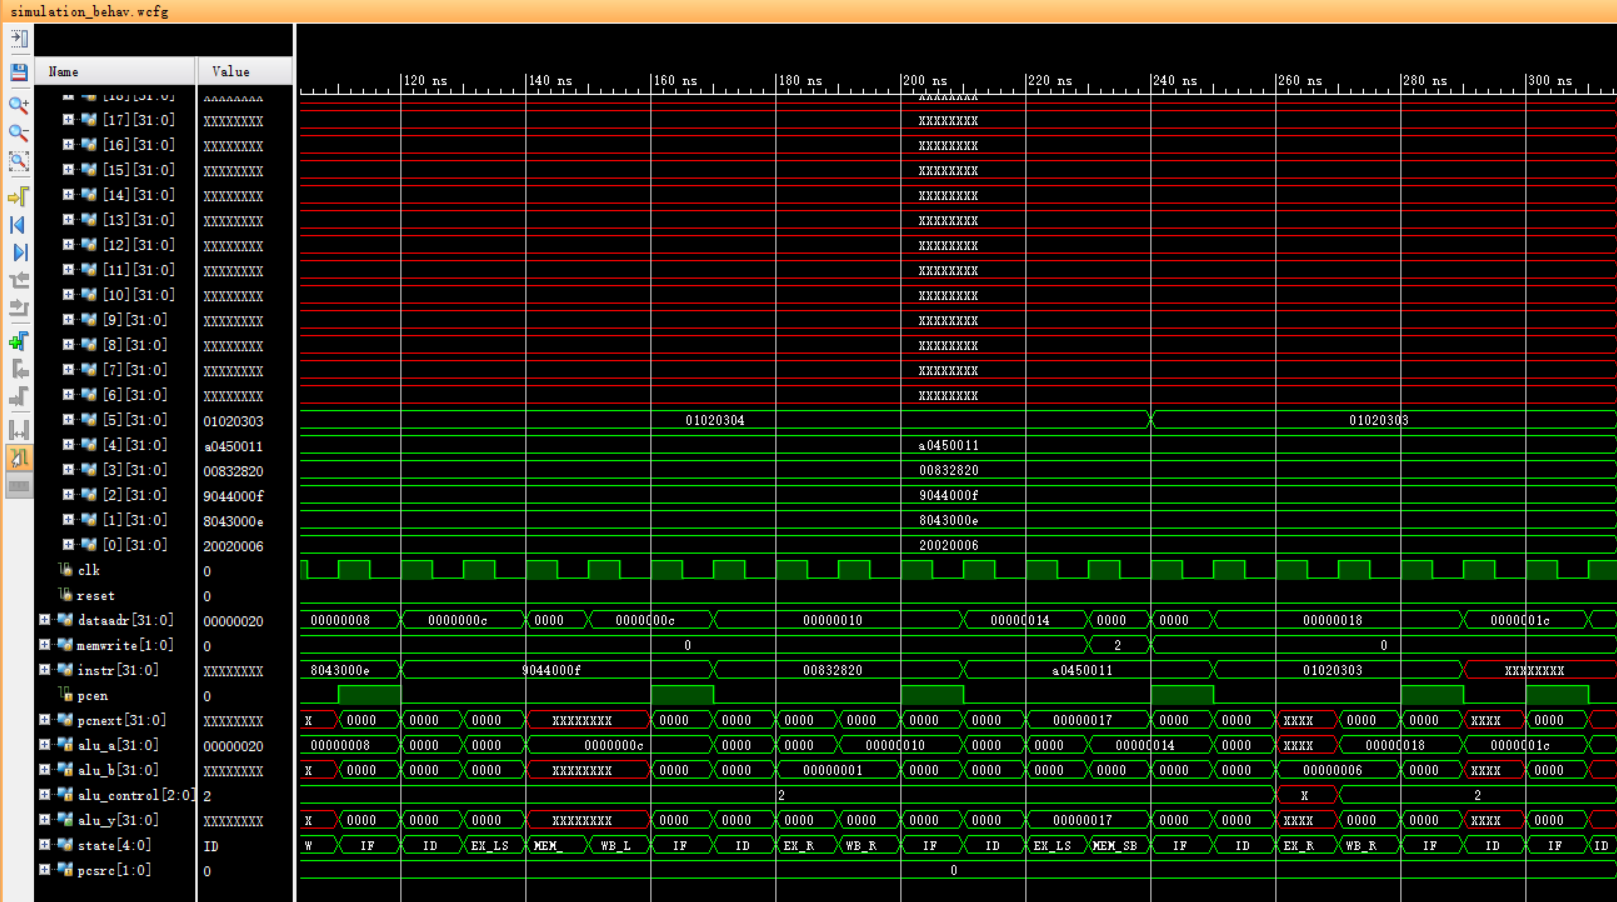
\includegraphics{C:/Users/will131/Documents/workspace/MIPS_V2.0/images/Simulation2.png}
\caption{}
\end{figure}

做完仿真测试之后,我对工程进行Synthesis和Implementation,最终生成二进制文件。工程的资源占用情况如下:

\begin{figure}
\centering
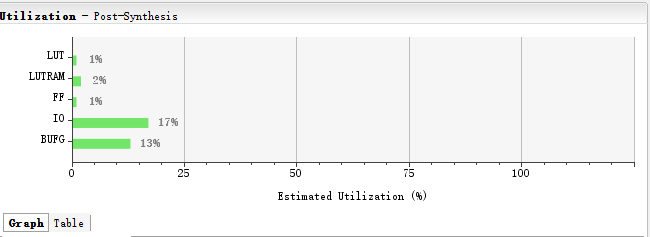
\includegraphics{C:/Users/will131/Documents/workspace/MIPS_V2.0/images/UtilizationGraph.png}
\caption{}
\end{figure}

\begin{figure}
\centering
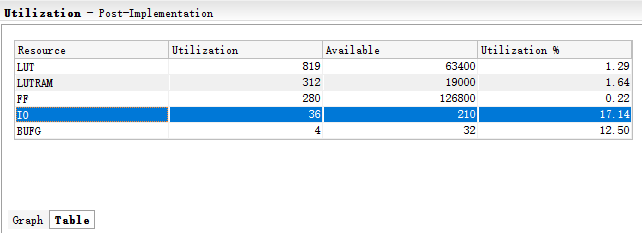
\includegraphics{C:/Users/will131/Documents/workspace/MIPS_V2.0/images/UtilizationTable.png}
\caption{}
\end{figure}

时钟情况如下:

\begin{figure}
\centering
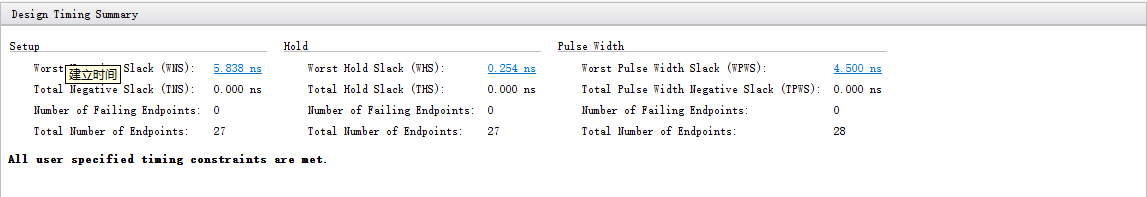
\includegraphics{C:/Users/will131/Documents/workspace/MIPS_V2.0/images/Timing.png}
\caption{}
\end{figure}

\subsubsection{八、演示设计}\label{header-n2020}

由于所有的模块都有相同的clk和reset信号控制,我用两个开关来绑定这两个信号,从而可以随时选择重新执行程序或者\textbf{暂停程序}的执行。为了方便在Nexys4实验板上展示我的项目,我还实现了在8位7段显示管上显示32位数的功能(每个7段显示管表示0-f之间的一个\textbf{十六进制位}),用于显示程序的各种信息。

在一般情况下,6、7位为你查看\textbf{寄存器的序号}(0-31),4、5位显示的是那个\textbf{寄存器的值}的低两位,2、3位显示的是\textbf{PC的值},0、1位显示的是当前\textbf{状态机的状态}(状态-序号对应表见states.txt)。其中寄存器的序号使用开关组成二进制数进行选择。当存储器被写入的时候,屏幕上会出现形如EExyEEzw的信息,表示存储器第xy个字被写入了zw(可能只写其中的某个Byte)。我们还可以通过开关(和寄存器检查的开关组一致)选择\textbf{存储器检查模式},以字为单位检查存储器中任意地址上的值。另外,为了便于查看关键的程序执行,我还实现了用开关选择\textbf{快速运行}与\textbf{常速运行}两种模式。

具体的代码实现见onboard.sv,详细的使用说明见states.txt.

\subsubsection{九、后记}\label{header-n2027}

由于前面有其他课程的作业,后面还是有其他课程的作业,我这次实验的工作主要都集中在这一个星期里。对于32位改64位的调研已经基本完成了,如果这两天有空我会快速做出64位版本的多周期MIPS;如果没有时间的话,我会在流水线版本里实现64位的MIPS。

\end{document}
